\chapter{A new device to record wrist movement in free living humans}
\label{Chap:Methods}
This section covers the actual methods and techniques used to create our Wrist 
Motion Activity tracker. We discuss the various hardware techniques used to 
create the device (\ref{Sec:Hardware}). This includes different sensors available,
picking the right one for our purpose and then prototyping a device. Note that
since the wrist activity motion tracker is to be mounted on the wrist, it needs
to be a small device that can be worn for a long interval\footnote{At least
16 hours} without discomfort to the user. This means that it also needs to
have a long battery life, which is dictated by two factors: The size of the 
battery, and the current consumption of the parts on the device.

Then we discuss the software techniques and code used to create the device or the software to interact with it that runs on a desktop computer. Two different software were used to analyze the data from the device. This is briefly discussed in the Software section (\ref{Sec:Software}). Our ultimate aim to count the number of bites in each meal has made us look towards the rotational and linear movements of the wrist. This in turn has led us to consider linear acceleration and angular rotation data which is sensed by an accelerometer and a gyroscope respectively.

\section{Hardware Selection}
\label{Sec:Hardware}
Our planned device design for the all day wrist motion activity tracker revolves around a system of sensors that are polled at 15Hz by a microcontroller. This data is logged throughout the day, after which it is transferred to a computer for processing. Once the data for a day has been logged, the device is connected to a computer and data from the memory chip is dumped to a computer where it can be analyzed. As all this happens throughtout the day, we need some kind of display to inform the user of the status of the device.

To create the prototype device, different prototype breakout boards were used (\ref{Sec:Breakouts}). These boards allow rapid prototyping by hooking up components using wires. This reduces any time spent to solder an Integrated Circuit to the PCB or to understand its typical application circuit components. Next, we consider the different devices used to create our wrist motion activity tracker. We would need a power source in the form of a battery (\ref{Sec:Battery}), sensors to measure acceleration (\ref{Sec:Accelerometer}) and angular velocity(\ref{Sec:Gyroscope}), a memory chip (\ref{Sec:Memory}) to store data from the sensors and a microcontroller (\ref{Sec:MicroController})to control this system and act as a communication channel between the different devices. To connect this device to a computer, we would need a translator. We use a USB to UART bridge (\ref{Sec:FT232}) to accomplish this.

With all these components available, we would have to connect them together correctly, which is explaining in the Circuit Design section(\ref{Sec:CircuitDesign}). Once the design has been tested, it is laid out as a PCB design using EAGLE PCB, and then fabricated. This PCB would then need the IC's soldered to it, and we discuss the two methods used to do so (\ref{Sec:Soldering}).

We recap that we have two strong requirements for our device, and all hardware decisions must consider these:
\begin{itemize}
  \item Device Size
  \item Device Power Consumption
\end{itemize}
With this in mind, we look at the different hardware in our device in the next section.

\subsection{Sensors}
\begin{figure}
\begin{center}
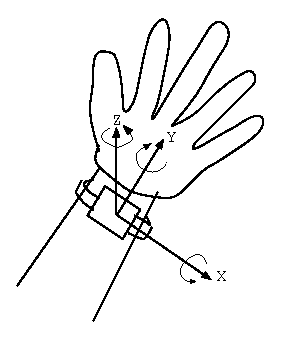
\includegraphics{images/HandAxis.eps}
\caption{Orientation of axes in the IMU when mounted on the wrist}
\label{fig:AccAxis}
\end{center}
\end{figure}
Since we want to log acceleration and rotation data, we looked at the different sensors available in the market and their sizes. The clear winner was a category of sensors called MEMS sensors. MicroElectroMechcanicalSystems based sensors are small devices ranging from about 4 mm\textsuperscript{2} to  25 mm\textsuperscript{2}. Our device design uses an MEMS gyroscope and accelerometer in a single electronic chip to sense movements. This chips may also be called the IMU or the Inertial Measurement Unit. The orientation and axes for this chip is shown in figure \ref{fig:AccAxis}.

\subsection{Accelerometers}
\label{Sec:Accelerometer}
Accelerometers are devices that sense linear acceleration. In the case of our device we would like to measure the linear acceleration in all three Cartesian co - ordinate axes, X, Y, and Z. This will allow us to track the movement of the wrist in free living humans as their hand moves around in free space. Figure \ref{fig:AccAxis} shows how the axis of the sensor are oriented for our device.

To understand how an accelerometer works, we imagine a system devised of a spring connected to a fixed surface at one end as shown in figure \ref{fig:HookeSpring}, and an object with a mass M at the other end. Since springs are governed by Hooke's Law, we can use that to explain its behavior. Hooke's law states that to extend or compress a spring by distance X, the force required is proportional to X, or mathematically as given in equation \ref{Eqn:HookesLaw}.
\begin{equation}
\label{Eqn:HookesLaw}
F = -kX 
\end{equation}
where F is the force required, X is the distance the spring is extended or compressed from its equilibrium position, and k is the spring constant for a particular spring.
\begin{figure}
\begin{center}
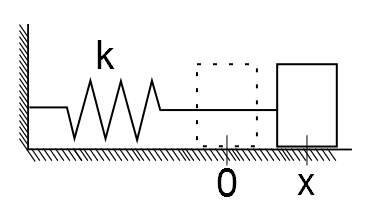
\includegraphics{images/HookesLaw.png}
\caption{Example of a spring system}
\label{fig:HookeSpring}
\end{center}
\end{figure}

\hfill \\
We also have Newton's Second Law of Motion which states that the force applied on a body with constant mass produces a proportional acceleration.Mathematically, Newton's Second Law of motion can be expressed as given in equation \ref{Eqn:Newtons2ndLaw}.
\begin{equation}
\label{Eqn:Newtons2ndLaw}
F = ma 
\end{equation}
where F is the force, m is the mass of the body, and a is the acceleration produced. Combining the two equations, we can solve for acceleration using the result in equation \ref{Eqn:HookeAcc}.
\begin{equation}
\label{Eqn:HookeAcc}
a = \frac{-kx}{m} 
\end{equation}
However, consider the fact that the spring constant k and mass m are constant in the equation above. This means that acceleration a is inversely proportional to the displacement x. Knowing this, new MEMS accelerometers are very simple systems consisting of small mechanical parts that measure the displacement and output an acceleration based on this.
\hfill

We must remember that since the sensor is measuring force, that gravity is always acting on the device, and due to this, a reading of 1g will always be read on the Z axis for the "earth" system. If there are no rotational movements, we know which direction gravity is acting in, and can subtract this from the readings obtained from an accelerometer.

\subsection{Gyroscopes}
\label{Sec:Gyroscope}

Gyroscopes are devices used to measure angular movement. In our case, we use MEMS gyroscopes to measure angular velocity in three axes, X, Y and Z (as shown in figure \ref{fig:AccAxis}). How a gyroscope works in explained in ~\cite{Web:SparkfunGyros}. We will review the same here.
\begin{figure}
\begin{center}
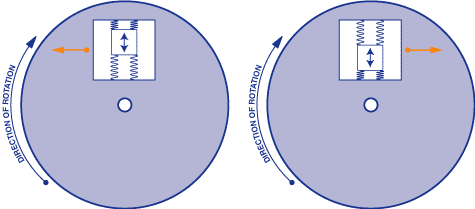
\includegraphics{images/GyroWork.png}
\caption{Internal Working of a Gyroscope}
\label{fig:GyroDiag}
\end{center}
\end{figure}

An MEMS gyroscope contains a small mass that oscillates inside it as shown in figure \ref{fig:GyroDiag}. When the gyroscope rotates, the oscillating mass is displaced between two oscillations. This change in location is converted into a very low current, that is then amplified (and converted to a voltage) by a microcontroller inside the gyroscope integrated chip.

\subsection{Accelerometer and Gyroscope Device selection}
There are a variety of MEMS accelerometers and gyroscopes available in the market with different specifications. Our purpose was to pick the most suitable device for logging wrist movement data. We will first look at the different parameter's that we have for MEMS devices. These parameter's are referenced from Analog Devices' website\footnote{\href{http://www.analog.com/en/content/td_accelerometer_specifications_definitions/fca.html}{Analog Devices - Accelerometer Specifications - Quick Definitions. Last accessed October 2014}} :

\begin{description}

\item[Output] \hfill \\
The output of the sensor can be analog or digital. For an analog device, the output is a voltage corresponding to the detected measurement. This means that an acceleration between -A$_{max}$ to +A$_{max}$ would be output as a voltage between V$_{dd}$ and V$_{cc}$. Each output would have its own pin to output a signal. A digital device on the other hand, would use some kind of communication protocol. The device usually has registers or a memory stack that can be read using a protocol like I$^2$C (also known as TWI) or SPI. Using this protocol, a master device (microcontroller) can poll the slave (accelerometer) to read its memory.

\item[Output data Rate] \hfill \\
This defines the rate at which data is sampled and then output by the device. In analog accelerometers, this represents how often an accelerometer updates its output voltage in response to the measured acceleration. In digital accelerometers, this represents how often the register storing the value of the acceleration is updated. Our required data rate is of 15Hz for sufficiently accurate monitoring of wrist movements.

\item[Package type and Size] \hfill \\
Since the device is mounted on the wrist, space and volume is at a premium. Most MEMS devices are catered to the consumer electronics market, and used in small devices like mobile phones and smart watches. Due to this, there is constant innovation in the market with regards to the size of the integrated chip's footprint. Packages like LGA (Land Grid Array) and QFN (Quad Flat No - Lead) are used. These packages usually lack pins and are surface mounted to reduce the footprint on a PCB. An example of this is the IMU that we used in our device, the MPU 6000 produced by Invensense Inc. An image from Sparkfun.com~\cite{Image:SparkfunMPU6000}  (see figure \ref{fig:MPU6000Size}) shows the size of the chip compared to a quarter.

\begin{figure}
\begin{center}
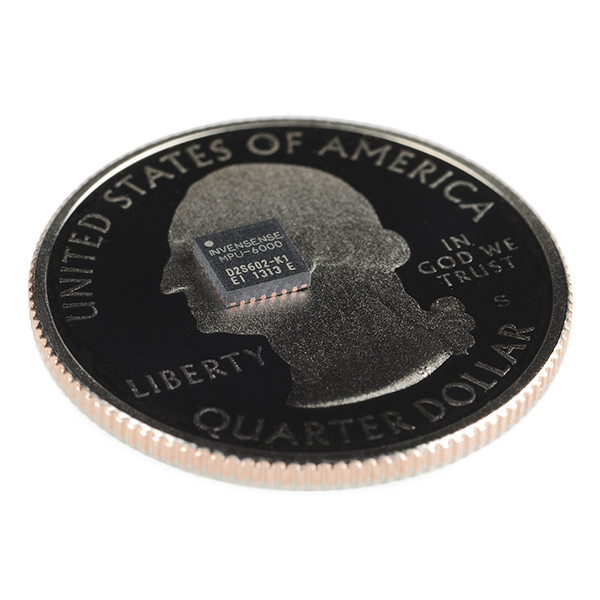
\includegraphics[width=0.5\textwidth]{images/MPU6000Size.jpg}
\caption{The MPU6000 IMU lying on an American Quarter for size comparison.}
\label{fig:MPU6000Size}
\end{center}
\end{figure}

\hspace{2em}
\item[Measurement Range] \hfill \\
This defines the range of measurement supported by an IMU's output specifications. For an accelerometer, the range is usually defined in g's, where 1g = 9.8 m/s\textsuperscript{2}. This is the greatest amount of acceleration that can be measured and accurately represent as an output. A larger acceleration maybe incorrect or capped at the maximum value. For example, the MPU-6000 has four modes with measurement ranges from $\pm{2}$g to $\pm{16}$g. The measurement is not the breaking point for the device. A higher acceleration of 17g may not break the accelerometer, but will not be reported correctly. This value is actually defined as the Absolute Maximum Acceleration.
 
Human motions are typically contained within 2g's of acceleration. With this fact, our options for accelerometers is fairly large considering that most MEMS accelerometers aimed at consumer electronics will have a measurement range of 2g's. 
\hfill 
\item[Current Consumption] \hfill \\
The power drained by the device is a huge factor for us. MEMS accelerometers are fairly low power devices. The LIS344ALH accelerometer used by Drennan in \cite{drennan2010assessment} typically consumed 650 $\mu{A}$ of current when operating and a maximum of 5$\mu{A}$ when in sleep mode. Gyroscopes on the other hand tend to consume a very high amount of current. \cite{drennan2010assessment} used two gyroscopes, each consuming 6.8mA. This means that on a standard coin cell battery that has a size of 90mAh, the gyroscopes would run for about 7 hours, a very short lifetime.

\item[Number of Axes] \hfill \\
As MEMS technology has improved, the sensors abilities have improved. Early accelerometers would sense acceleration across a single axis. With current technology, most accelerometers and gyroscopes can measure across all three axes. Inertial Measurement Unit's are available that pack not only an accelerometer and a gyroscope, but also a magnetometer for more accurate measurements. This greatly reduces the current consumption against a scenario where multiple devices are being used. We will not be using a magnetometer for our work.
\end{description}
\inputfile{tables/SensorTable.tex}
With these parameters, we compared a few of the options available in the market in September 2013. Table \ref{Tab:SensorCompTable} shows the different product names versus their important parameters. The first three products are the ones used in \cite{drennan2010assessment}.
Based on these different parameters and comparing with \cite{drennan2010assessment}, we have selected the Invensense MPU-6000. The device contains both, a 3-axis accelerometer and a 3-axis gyroscope. It features three 16-bit analog-to-digital converters each for both these devices to digitize the sensor outputs. This data is stored in internal registers that can be accessed using I$^{2}$C at 100kHz or using SPI at 1Mhz. An on-chip buffer allows storing bursts of readings, which can be read in bursts by a master device. The device operates at a voltage of 2.375V to 3.46V, which would mean operation on most Lithium Ion battery. An operating current of 3.8mA means that the device can operate for roughly 24 hours on a standard coin cell battery. This makes the MPU 6000 very suitable for our requirements.

\subsection{Breakouts}
\label{Sec:Breakouts}
Newer integrated chips are packaged very densely, and have very small pins to connect to a PCB. With surface mount technology, it is possible to solder these devices to PCB's, however it is very hard for hobbyists to do so, because of the lack of expensive equipment. Electronic part retailers provide products in the form of Breakout boards, which means that they provide PCB's with the integrated chip soldered. These PCB's have pins to connect to that can be used conveniently. In effect, a breakout board converts pin - less packages like BGA (Ball grid array) and LGA (Land grid array) to DIP (Dual inline package).
\begin{figure}
\begin{center}
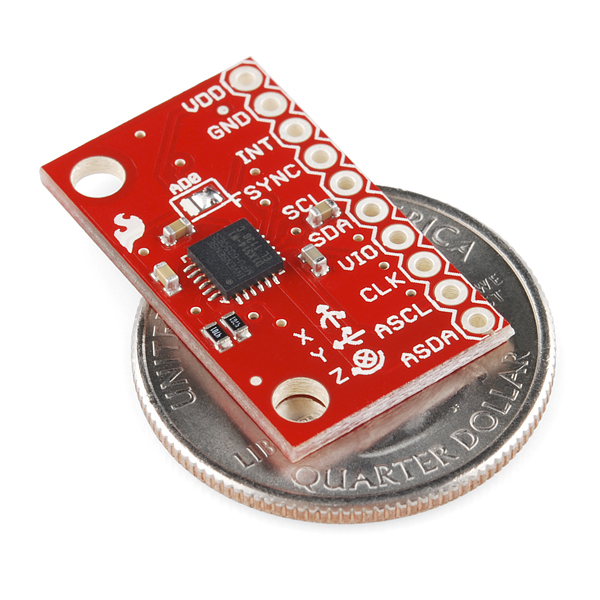
\includegraphics{images/MPUBreakout.jpg}
\caption{A breakout board containing the MPU 6050 chip. Quarter shown for comparison. Image from Sparkfun.com}
\label{Fig:MPUBreakOut}
\end{center}
\end{figure}

These breakout boards are easier to prototype with, and allow modular creation of a complete circuit. Although we have selected the MPU 6000, we still have to work it into our circuit and ensure that it will work in our device. To do so, conventional methods would require us to first solder this IC to a PCB containing the other components, and then programming a microcontroller to read from the sensor. However, PCB fabrication and soldering can be expensive, and are not a viable option during the prototype period. PCB manufacture can also take a considerable amount of time (up to a month), and is not a feasible strategy to work with. To prototype and test the sensor without fabricating a complete PCB, we decided to use a Breakout board containing the sensor. Figure ~\ref{Fig:MPUBreakOut} shows an example of a Breakout board. The image was sourced from ~\cite{Web:SFBreakout}.

\subsection{Memory}
\label{Sec:Memory}

The information sensed by the sensors has to be logged, and then processed by a computer. We could either store this information or transmit it wirelessly as it is gathered. For a system planned to read sensors at 15Hz, and logging data for 24 hours, we estimate the amount of data as shown in Equation \ref{Eqn:DataAmount}

\begin{equation}
\label{Eqn:DataAmount}
Data = 24~hours * \dfrac{60~minutes}{hour} * \dfrac{60~seconds}{minute} * \dfrac{15~polls}{second} * \dfrac{6~sensors}{poll} * \dfrac{1~byte}{sensor~poll}
\end{equation}

\begin{equation}
\label{Eqn:DataAmount2}
Data = 7,776,000~Bytes = 7,593.75~KiloBytes
\end{equation}

We do not consider wireless transmission in our case. The device would have to transmit data to another device which it would be paired to. The paired device would need to remain in wireless connectivity range to store this data. This adds another device to our solution, so we do not consider it. 

To store the roughly 6 Megabytes of data, we need some kind of memory. We see in \ref{Sec:MicroController} that our microcontroller only has a Flash Memory of 48KB. This would mean we need a memory to store the data during the interval that the user is wearing the device. This data can then be transferred to a computer from the memory once we have a connection between the two.

We compared the available options in the market. Most memory chip's are sold in power's of 2, so we would have to look at devices close to 8 Megabytes or 64 Megabits in design. A search on Digikey in October 2013 showed that there were very limited options in the Flash memory market that would support such a high density of memory. The options were further limited by the fact that we required a small footprint that we could add to our wrist mountable device. Options typically had parallel input / output which meant they had close to 28 pins.

Atmel's memory division had just released AT45DB642D, a 64-megabit 2.7V Dual-interface DataFlash memory chip. This chip would support the amount of memory we required, and ran on a single 2.7V - 3.6V supply, which our system worked on. This chip also supported SPI, the same protocol that was being used by the sensors in our circuit. SPI allows us to use the same bus for data communication and clock, while using one extra line for each device's slave select pin. Figure \ref{Fig:SPISLAVES}, courtesy of \cite{Web:WikiCBurnett} shows how two slave devices can connect to an SPI master. This means that we could reduce the number of I/O pins used in our microcontroller, and also reduce the number of tracks created on our PCB for data communication.

\begin{figure}
\begin{center}
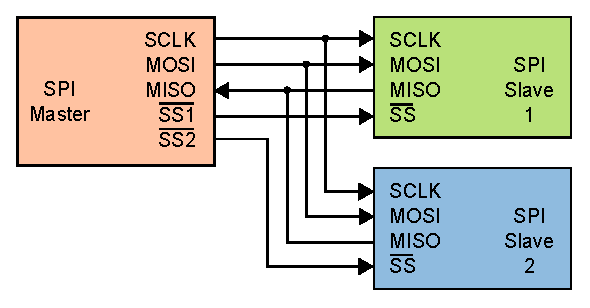
\includegraphics{images/SPI_SLAVES.eps}
\caption{An SPI system with two slaves on the same bus.}
\label{Fig:SPISLAVES}
\end{center}
\end{figure}

The chip was made available in an unconventional CASON package, which is a surface mount device. This means we would have to solder the chip before it could communicate with a microcontroller. To avoid the delay incurred because of PCB fabrication (which can take up to two weeks), we jerry rigged the chip. After flipping it upside down, so that its pins are exposed, we soldered strands of a multistrand wire to each of these pads. These strands were then soldered through a dot matrix PCB, allowing us to use the new unit as a Pin Through Hole device. This required careful handling of the chip with a dextrous hand, and was done under a microscope. Figure \ref{Fig:CASON} shows the result. 

\begin{figure}
\begin{center}
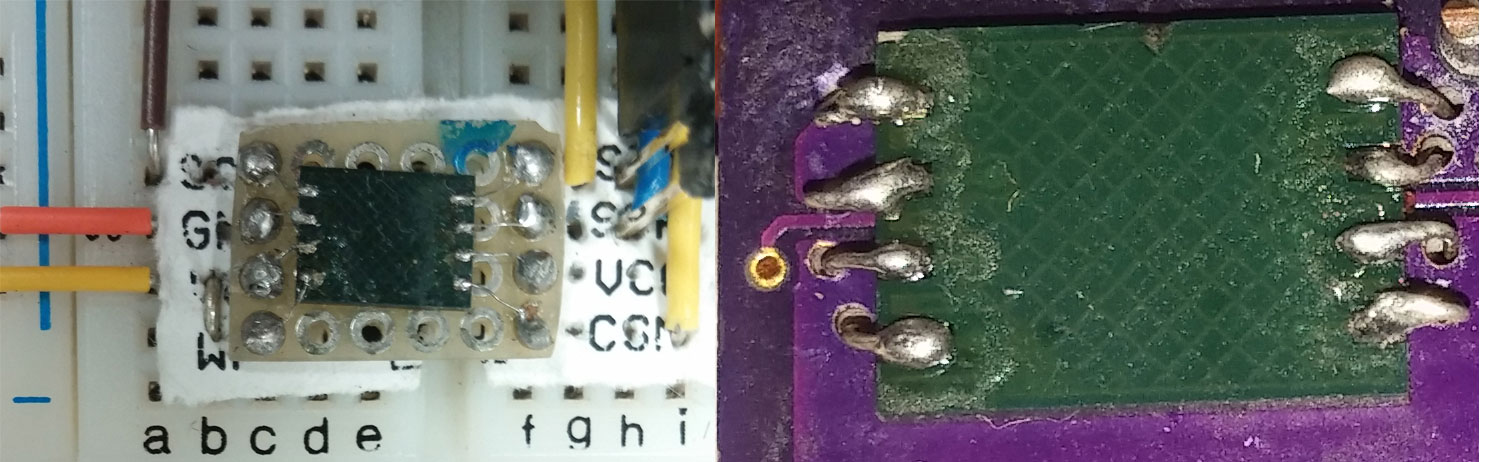
\includegraphics[width=1.0\textwidth]{images/CASON.jpg}
\caption{Two examples of flipping over a CASON chip and soldering wires to it's pads.}
\label{Fig:CASON}
\end{center}
\end{figure}
 

\subsection{Microcontroller}
\label{Sec:MicroController}

The sensors we discussed in the previous section cannot function on their own. They are primarily slave devices that can be requested for data. To get this data, we require a master device, which we have in the form of a microcontroller. Our microcontroller would need to support the communication protocol used by our sensors and memory chip. It would also need to have a sufficient memory to be able to temporarily buffer sensor data before it is flushed to the external memory chip. 

Several manufacturers provide microcontrollers that we can use, however, our priority of low current is what will separate the different microcontrollers, and help us pick the right one for our device. We considered the different wrist based devices on the market and realized that the MSP430 family of microcontrollers greatly dominates this market segment. The MSP430 Brochure \cite{instruments2009msp430} lists roughly three hundred parts that can be picked from, categorized as:

\begin{itemize}
  \item Low Power FRAM Series
  \item Value Line Series with limited components
  \item F - Family with increased integration and performance
  \item F - Family with an integrated LCD driver
  \item F - Family with high frequency operation (up to 25 Mhz)
  \item CC430 Series (Microcontroller with integrated RF chip)
\end{itemize}

When selecting our chip,
we needed one that would allow future expansion with regards to the capabilities of the wearable monitor.
\cite{Web:ShimmerHome} uses the MSP430F1161 which looks like a good fit for our device. 
However, almost the entire MSP430 family is pretty close to what we might need.
Our microcontroller would need SPI or I$^2$C support so that it can communicate with the memory chip and our sensor.
The MSP430F1161 lacks any module that can communicate over the SPI protocol,
which would mean we would have to implement a software based module,
increasing the complexity of the device.
The microcontroller would also need to have a buffer large enough to store
a sizable amount of data before it would need to be flushed to the memory chip.
After combing through the brochure, we found the first parts with SPI support and
a minimum SRAM of 2048 bytes in the MSP430F24X series. This sub-family of devices had
the following characteristics (as seen in \cite{msp430F24xfamily})

\begin{itemize}
	\item Low Supply-Voltage Range, 1.8 V to 3.6 V
	\item Active Mode Current Consumption: 270 μA at 1 MHz, 2.2 V
	\item Standby Mode (VLO) Current Consumption: 0.3 μA
	\item Four Universal Serial Communication Interfaces supporting SPI and I$^2$C.
	\item Two 16-Bit Timers with multiple compare registers.
\end{itemize}
We select the MSP430F248 as our microcontroller. This chip comes with a 48KB+256B Flash Memory, and 4KB of RAM. Assuming our program size would not be more than 1 KB, this would allow us to buffer about 3KB of data from the sensors before flushing it to the external memory, allowing the memory to remain in sleep mode for a large amount of time.

\subsection{MSP 430 Target Board}
\label{MSP430Target}

\begin{figure}
\begin{center}
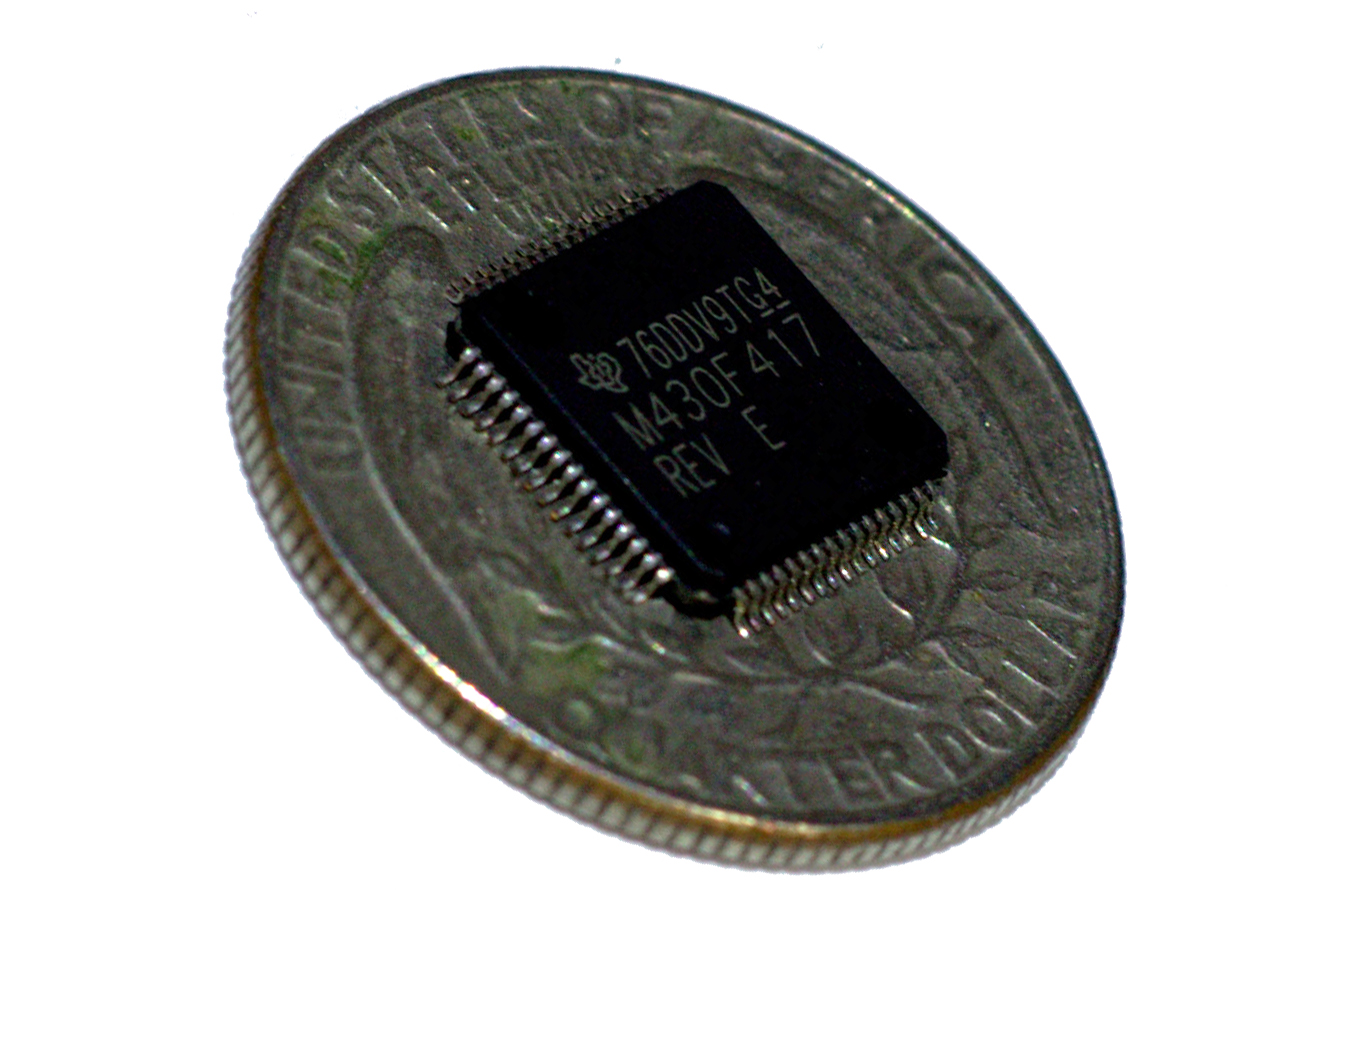
\includegraphics[width=0.5\textwidth]{images/QFPFoot.jpg}
\caption{The MSP430F248 integrated chip, with a quarter to show scale.}
\label{Fig:QFPFoot}
\end{center}
\end{figure}

Like our sensors, the MSP430F248 also comes in a surface mount package.
The footprint is shown in Figure \ref{Fig:QFPFoot}
and known as the QFP\footnote{Quad Flat Package} design.
This package does have pins, but they are not long enough to pass through a PCB.
Instead they have to be mounted on the PCB.
It is very hard to design a complete system without bugs and if we would design a PCB
while writing microcontroller code at the same time,
it would not be easy to debug an error because we would not know if the error
is in the hardware design or the software code. Texas Instruments' understands this,
and provides a 64-Pin Target board for its microcontroller. This target board has
a ZIF\footnote{Zero Insertion Force} socket that accepts the 64-Pin QFP chip,
and breaks out its pins. This means other devices can be connected to the board with ease,
allowing us to program the microcontroller without having soldered it.
\begin{figure}
\begin{center}
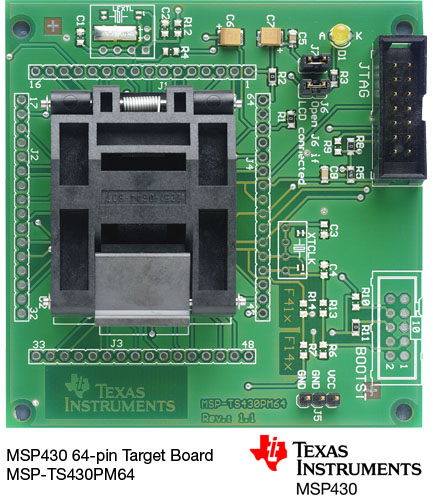
\includegraphics[width=0.5\textwidth]{images/mspts430pm64.jpg}
\caption{The MSP430 64-Pin Target Board. Image provided by Texas Instruments}
\label{Fig:MSPTarget}
\end{center}
\end{figure}

Figure \ref{Fig:MSPTarget} shows us what the MSP430 Target Board looks like, with the socket in the center. You can see a connector in the top-right of the figure, which is labeled JTAG. The socket is surrounded by holes on all sides which connect to the microcontrollers pins, allowing for easy connections. The target board also allows for a crystal to be soldered next to the microcontroller if the programmer wants to use the Low Frequency Clock based on an external crystal. We use this crystal for and accurate clock when polling our sensors, and also when communicating with a host computer as we will see in section \ref{Sec:FT232}.

\subsection{MSP430 Flash Emulation Tool}
\label{Sec:MSP430FET}
Now that we have a microcontroller selected, and a target board that allows us to easily set it up electrically, we need a way to program it with our code. The MSP430 series of microcontrollers are programmed by using JTAG using 4 wires. Modern computers usually lack a serial or parallel port for communication, so Texas Instruments provides programmers with the MSP430 Flash Emulation Tool. This tool (seen in Figure \ref{Fig:MSP430FET}) connects to a desktop computer through USB, and the other end connects to a standardized JTAG connector, as seen in \ref{Fig:MSPTarget}. 
\begin{figure}
\begin{center}
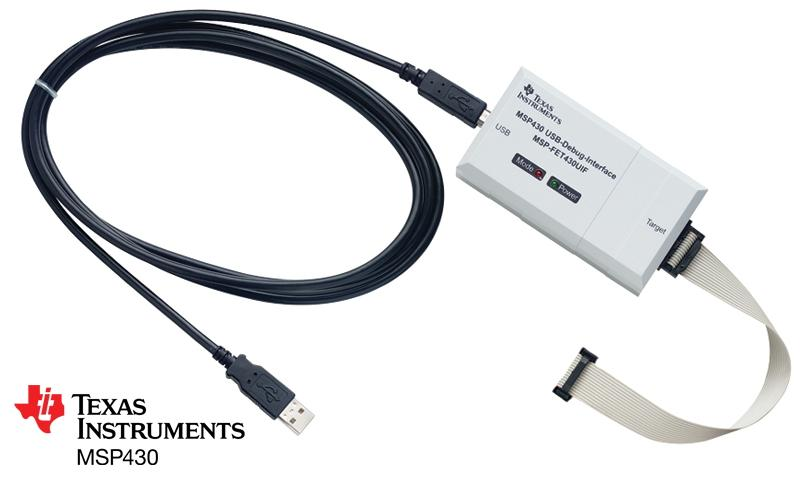
\includegraphics[width=0.5\textwidth]{images/MSP430FETUIF.jpg}
\caption{The MSP430 Flash Emulation tool. Picture courtesy Texas Instruments}
\label{Fig:MSP430FET}
\end{center}
\end{figure}

The tool also supports powering the system it is programming, so we were able to program our microcontroller without an external power source. Once we had our battery selected, a jumper on the MSP430 Target Board allowed us to disable the power supply of the Flash Emulation Tool. The FET can be used by various software, paid and free. For our use, we picked IAR's Code Composer Studio as it was available free of cost to students. Through the MSP430FET, IAR supports not only programming and flashing the microcontroller, but also debugging the code while it is running. This feature enabled us to fix multiple bugs in a short amount of time, something that would be hard to do without the debugging capabilities. We can also inspect different sections of the memory, allowing us to see live how the code is behaving.

\subsection{USB to UART Bridge}
\label{Sec:FT232}
With the above hardware in place, hopefully we have a system which reads from sensors and stores this data in the memory chip. Once data for an entire day is logged, we would like to transfer the contents of this memory to a computer where the sensor data can be analyzed for different patterns and behvaiours. Broadly speaking, there are two methods to transfer data, wireless and wired. Both these methods required parts that consume a current of about 18 mA when actively in use. Wireless transfer of data would consume power from the battery (unless a wire is connected to power the system), and assuming a speed of 115Kbps, this would take about 15 minutes to transfer. With an active current draw of 18mA for most wireless technologies, this would require a huge amount of power, something that the battery cannot sustain.
\begin{figure}
\begin{center}
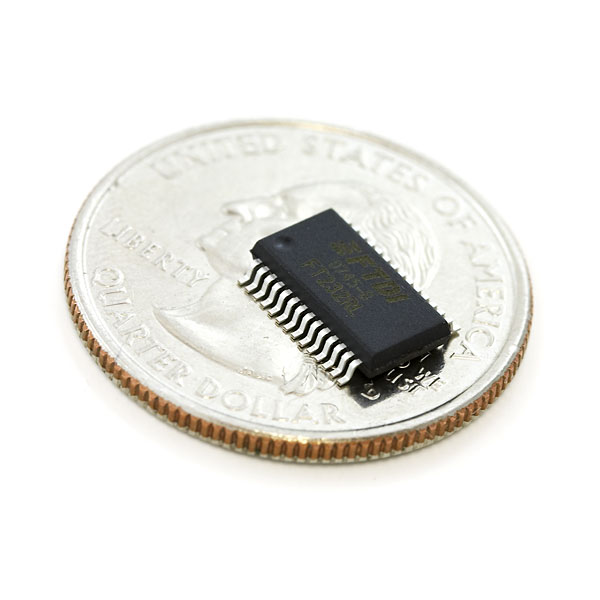
\includegraphics[width=0.5\textwidth]{images/FT232coin.jpg}
\caption{The FT232RL USB to UART bridge. Picture courtesy Sparkfun.com}
\label{Fig:FT232}
\end{center}
\end{figure}

We solve both these problems by using a wired connection to transfer data. As mentioned in \ref{Sec:MSP430FET}, modern computer systems only have the USB port as a viable way to communicate. Although some MSP430 microcontrollers have native USB support, those microcontrollers have an increased current consumption and are not viable to our purpose. Our selected microcontroller, the MSP430F248, does not have a native USB module, but does have other communication modules. The MSP430F248 has a UART, and a combined I$^2$C + SPI module that can be used for communication. Since we will be using SPI for communicating with the sensors and the memory chip, using UART is a good way to isolate modules being used at the same time. 

We looked for devices that would help convert communication in one protocol to another. Since SPI, I$^2$C and UART are all serial communication protocols, in theory, any device that can communicate in one of these protocols should be able to communicate in the other. However, a search on different devices in the market showed that USB to UART bridges are an easy way for microcontrollers to communicate with a computer. The device is detected as a virtual serial communication port to the operating system, and can be used as a regular serial port. Searching for USB to UART devices shows two primary contenders in the market segment, Silicon Labs and Future Technology Devices International (also known as FTDI). Both offer devices that have similar features and specifications. 

We need a device that would communicate easily with our microcontroller, the MSP430F248 and also be easy to prototype with. All of Silicon Labs' offered parts are only available in the QFN package, which means it would be hard to prototype using them. For this reason, we select FTDI's chip, the FT232RL (shown in figure \ref{Fig:FT232}. FT232RL has the following specifications (as seen in \cite{FT232Datasheet}):

\begin{itemize}
	\item Single chip USB to asynchronous serial data transfer interface.
	\item Data transfer rates from 300 baud to 3 Mbaud (RS422, RS485, RS232 ) at TTL levels.
	\item UART interface support for 7 or 8 data bits, 1 or 2 stop bits and odd / even / mark / space / no parity.
	\item Integrated +3.3V level converter for USB I/O.
	\item Available in compact Lead-free 28 Pin SSOP and QFN-32 packages.
\end{itemize}


\inputfile{tables/BatteryTable.tex}
\subsection{Battery}
\label{Sec:Battery}

While the wrist activity monitor is mounted and active, it needs a power source to operate on. Work done by \cite{Web:ShimmerHome} uses a single 450mah Lithium Ion Polymer battery. Similar batteries with higher capacities are found in mobile phones. We also see other batteries available in the market, with different characteristics based on the technology. Our wrist motion activity monitor requires a small battery which will supply a burst current of \~25mA when required. It should also hold enough power to supply current to the system for a minimum of 24 hours. Table \ref{Tab:BatteryCompTable} shows the different current battery types available in the market (as seen in \cite{Web:BatteryTable}), and their parameters.
\begin{figure}
\begin{center}
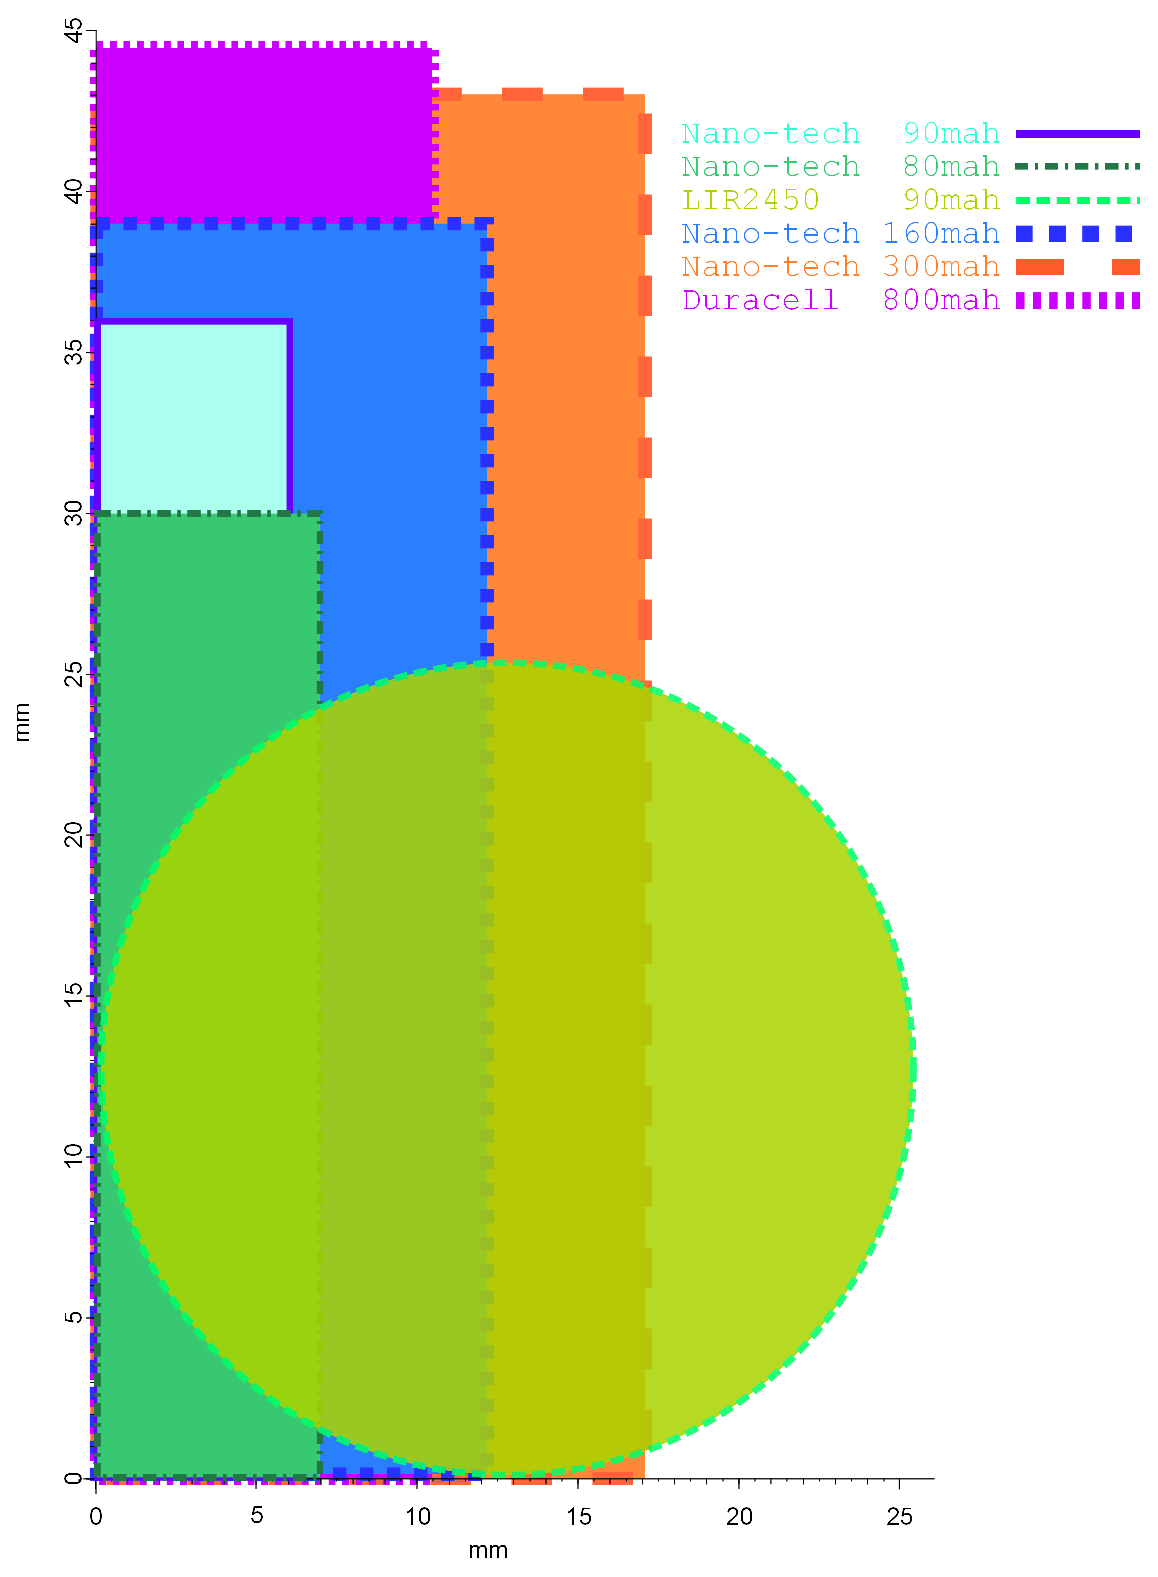
\includegraphics[width=0.5\textwidth]{images/battcompare.eps}
\caption{Top view profiles of the compared batteries.}
\label{Fig:BattComp}
\end{center}
\end{figure}
After looking at work done by \cite{Web:ShimmerHome} \& \cite{drennan2010assessment} we decided to consider Lithium-Ion batteries. Another field where Lithium Ion batteries are used is in flight. Since aerial vehicles need to have a low weight, batteries used in this application are high density and very efficient. We considered the batteries used in the fields mentioned above and compared some of them. The comparison is given in table \ref{Tab:Battery2}. A visual comparison of the different battery sizes is shown in figure \ref{Fig:BattComp}. As it can be seen, apart from the LIR2450, the battery sizes are somewhat similar,
so it may be possible to use a larger battery while still fitting our hardware in our case.

The width of the batteries would be an issue too.
As seen in section \ref{Sec:Case},
the case is curved along its median,
so a battery that was thicker could be accomodated if it was not too wide.
Emperical analysis showed that the Turnigy Nano-tech 160mAh battery
would fit with some modifications to the case (to allow a slightly thicker battery).

\subsection{Button}
\label{Sec:Button}
As with any consumer electronic device, we require the option to turn our device on or off. We might also want to provide our user with the option of erasing the memory for the device. This would require some kind of button (or buttons) to allow such interaction. We consider a scheme that required one button, with a state machine behaviour as given in table \ref{Tab:ButtonTable}. Based on this state machine behaviour, we recognize that a single pole single throw momentarily on switch is the most convinient device for our purpose. This button can be see in figure \ref{Fig:MomButton}. A momentary on button is similar to those seen on a remote, where the button switches on momentarily when pressed, and then deactivates as soon as pressure on it is released.
\begin{figure}
\begin{center}
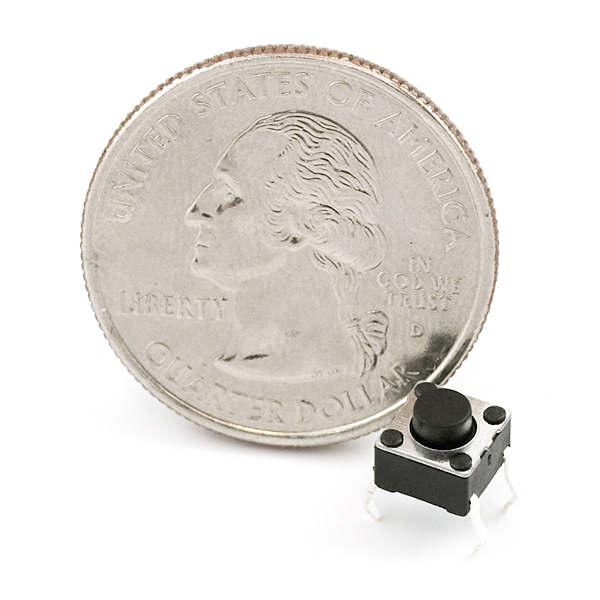
\includegraphics[width=0.5\textwidth]{images/MOMButton.jpg}
\caption{Example of a Momentary Switch. Picture courtesy Sparkfun}
\label{Fig:MomButton}
\end{center}
\end{figure}
\inputfile{tables/ButtonTable.tex}



\label{Sec:CircuitDesign}
\label{Sec:Software}

\subsection{Soldering}
\label{Sec:Soldering}
